\section{Neural network based caching policy} \label{caching_policy}

\subsection{Architecture} \label{architecture}

\begin{figure}[b!]
	\centering
	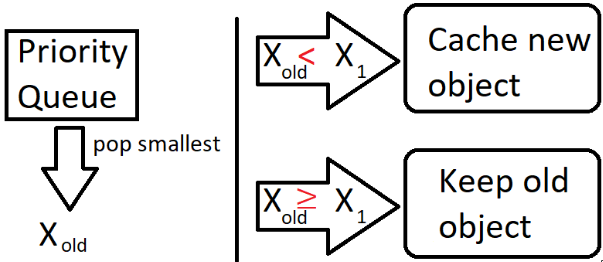
\includegraphics[width=0.75\linewidth]{pics/cache2.png}
	\caption{Usage of prediction by the policy.}
	\label{fig:cache2}
\end{figure}

After we have established the suitable neural network architecture for predicting content popularity, it is time to present a caching policy which uses such network. After each object request, it is possible to construct an input to the neural network, i.e. values $X_{-3}, \, ... \, , X_{0}$ and $t$, and obtain the predicted popularity $X_{1}$. After the prediction is made, the value $X_1$ is used to decide if the object should be put in the cache. The policy maintains a priority queue in which the key of each entry is the predicted popularity, and the values are IDs of the objects currently stored in the cache. When a new object is requested, and it has not been stored in the cache, the neural network predicts the popularity of the object in the future - $X_1$. Then, an object with the smallest predicted popularity is fetched from the priority queue, and its popularity is denoted as $X_{old}$. If the value $X_1$ is greater than $X_{old}$, then the old object is removed from the cache, and the new one is put in its place and into the priority queue. Otherwise, no change occurs.

With this design, a problem may arise - if the prediction of popularity for some object has been calculated to be very high, it may never be removed from the cache since it will never be fetched for replacement. A solution to this problem is to update the priority for a few random objects stored in the cache at each cache hit.

\subsection{Online learning} \label{online_learning}

One of the most important parts of a caching policy is to be able to perform well in different environments with different traffic patterns. That is why it is important to make the policy adaptable. In our case, such adaptability is provided by the ability of the neural network to continuously evolve by training on the newly arrived data. After the end of each time frame, it is possible to generate a new training dataset and use it to train the neural network, possibly asynchronously. But by training only on the latest data, we may encounter the problem of catastrophic forgetting \cite{16, 17}. In short, the issue is that by training only on the latest data the neural network will forget the information about the old underlying relations between input and output even though they still may be relevant for predictions. 

To overcome this issue, we incorporate a technique of keeping the training datasets of previous time frames and training the neural network also on them. But since they represent less relevant data, the error, which is backpropagated during the training of the neural network, is scaled down with a parameter $\alpha^M \text{, where } 0 < \alpha < 1 \text{ and } M$ is the distance from current time frame to previous time frames. In this way, the error on the most recent data will stay unchanged since the value of $M$ is $0$. Moving further in the past $\alpha^M$ becomes smaller and the influence of the old data is reduced. When $\alpha^M$ reaches a specific small value called forget threshold, the old training data becomes too irrelevant and can be removed from the memory. Using this approach with the value of $\alpha = 0.5$ and a forget threshold of $0.001$ it is required to store training datasets generated only for $10$ latest time frames while keeping the predictions made by the neural network accurate and relevant.

\subsection{Popularity prediction explained} \label{pop_prediction_explained}

\begin{figure}[b!]
	\centering
	\captionsetup{justification=centering}
	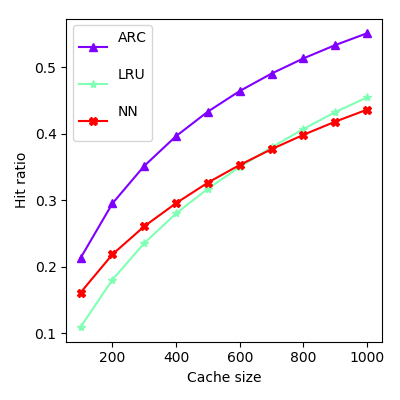
\includegraphics[width=0.5\linewidth]{pics/cache3.png}
	\caption{Hit rate evaluation on real-world data for different cache sizes when estimates for popularity in the next slot are used.}
	\label{fig:cache3}
\end{figure}

In the Section \ref{architecture} we were referring to the output of the neural network as predicted popularity and denoted it as $X_1$. There is a need for a more specific explanation. Using $X_1$ as the popularity of the object in the next time frame, as in the previous offline case, did not show good performance when evaluating the hit rate on real-world data described in Section \ref{real_data}. Figure \ref{fig:cache3} demonstrates the performance. The identified problem was that the prediction was made too far in the future. This lead to poor performance in the following two cases:

\begin{enumerate}
	\item If the object is popular in the current time window but then gets unpopular in the next, it would not be put into the cache, assuming the neural network correctly predicted low popularity in the next time frame. But since the current time window is not finished, and the object is still popular, a lot of cache misses will occur.
	\item Conversely, when the object is not popular but then gets popular, this object will take space in the cache even though it is not popular yet.
\end{enumerate}

To resolve this issue, we changed the scope of the value $X_1$. The desirable performance has been achieved using as true value the popularity evaluated at the end of the current timeslot (and not in the following one). We denote it as $X_1^{'}$. We would like to emphasize that the value $X_0$, which is passed as part of the input of the neural network, is not the same as $X_1^{'}$ since $X_0$ is the actual estimation of the popularity in the current time frame while $X_1^{'}$ is evaluated when the current time frame is finished, i.e. in the future. The improved performance is displayed in the Figure \ref{fig:cache4}. Probably it is still possible to improve the performance by fine tuning the parameters. 

\begin{figure}[h!]
	\centering
	\captionsetup{justification=centering}
	\begin{subfigure}[b]{0.49\linewidth}
		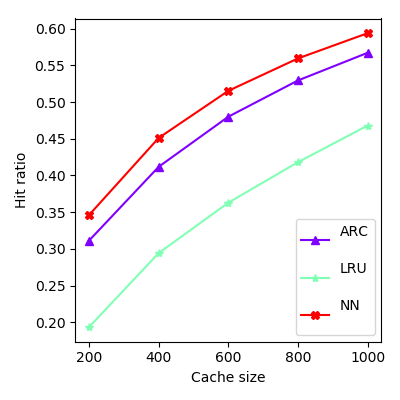
\includegraphics[width=\linewidth]{pics/cache4.png}
		\caption{5-day trace.}
	\end{subfigure}
	\begin{subfigure}[b]{0.49\linewidth}
		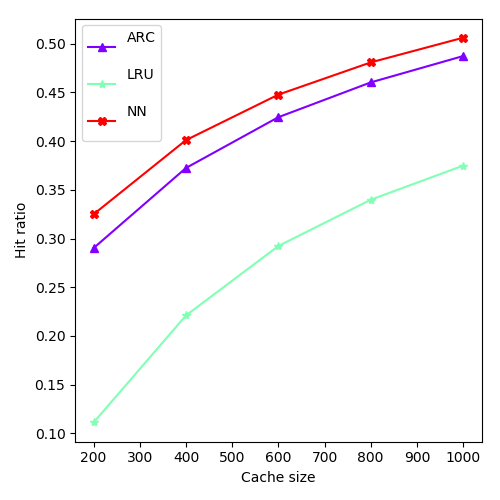
\includegraphics[width=\linewidth]{pics/cache4_2.png}
		\caption{30-day trace.}
	\end{subfigure}
	\caption{Hit rate evaluation on real-world data for different cache sizes after improvements.}
	\label{fig:cache4}
\end{figure}

\subsection{Parameter selection} \label{parameter_selection}

In Section \ref{pop_prediction_explained} we have shown that our NN-based caching policy achieves good performance on both of the real traces and overperforms state-of-the-art policy ARC for all cache sizes, as seen in the Figure \ref{fig:cache4}. Parameters there have not been selected carefully. In this section we will explore the optimal way to select the parameters.

\begin{figure}[t!]
	\centering
	\captionsetup{justification=centering}
	\begin{subfigure}[b]{0.49\linewidth}
		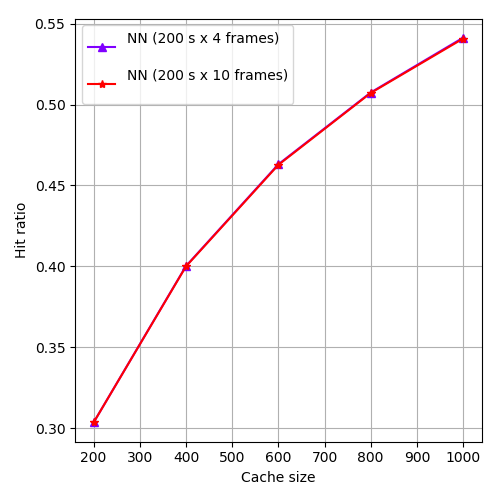
\includegraphics[width=\linewidth]{pics/cache5.png}
		\caption{5-day trace.}
	\end{subfigure}
	\begin{subfigure}[b]{0.49\linewidth}
		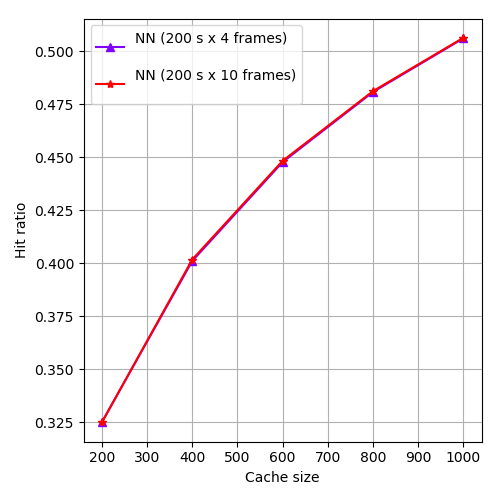
\includegraphics[width=\linewidth]{pics/cache5_2.png}
		\caption{30-day trace.}
	\end{subfigure}
	\caption{Comparison of hit rates obtained by evaluating proposed policy on real-world traces with fixed time frame size and different number of frames.}
	\label{fig:cache5}
\end{figure}

The first step we decided to check is the required number of time windows. To establish this experiment, we have fixed the length of the time frame at the value of 200 seconds and tested three configurations: 1) 2 time frames (previous + current), 2) 4 time frames (3 previous + current) and 2) 10 time frames (9 previous + current). The results of the experiment can be seen in the Figure \ref{fig:cache5}. As seen in the figure, the 10-frame curve and 4-frame curve closely follow each other while 2-frame curve trails a little behind. From this, we can conclude that it is enough to use 4 time frames for popularity predictions and there is no point in increasing this number since the improvement in performance not present or negligible. There is also no point in decreasing the number of frames since the performance in terms of hit rate decreases.

Then, we have to determine the optimal way to select the length of the time frame. We have established an experiment trying to evaluate this value. We have fixed the number of windows to be 4 and tested different configurations of time window size with cache sizes:

\begin{itemize}
	\item Time frame sizes: 3 s, 10 s, 50 s, 200 s, 1000 s.
	\item Cache sizes: 200, 400, 600, 800, 1000.
	\item Trace length: first 50 000 000 requests from both real traces.
\end{itemize}

\begin{figure}[t!]
	\centering
	\captionsetup{justification=centering}
	\begin{subfigure}[b]{0.49\linewidth}
		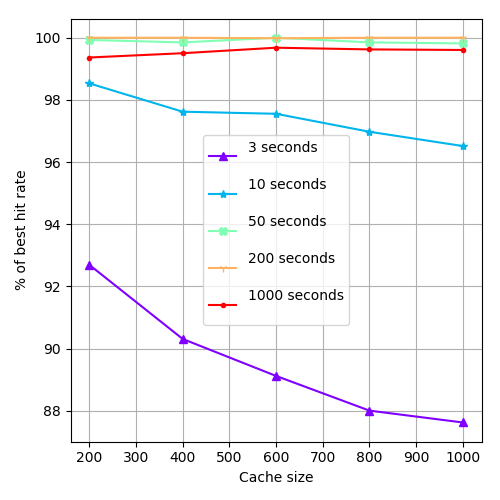
\includegraphics[width=\linewidth]{pics/cache6.png}
		\caption{5-day trace.}
	\end{subfigure}
	\begin{subfigure}[b]{0.49\linewidth}
		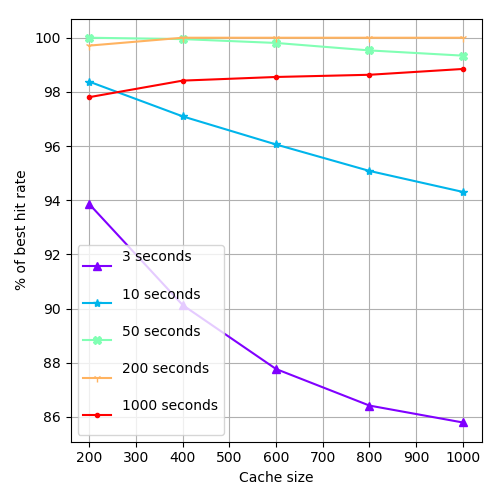
\includegraphics[width=\linewidth]{pics/cache6_2.png}
		\caption{30-day trace.}
	\end{subfigure}
	\caption{Comparison of hit rates obtained using modifications of the proposed policy with different sizes of time frame.}
	\label{fig:cache6}
\end{figure}

The experiment showed that the size of the window has a stronger influence on the performance than the number of windows. For both traces, the size of 200 s showed the best performance for all cache sizes with the exception of cache size 200 on the 30-day trace, as you can observe on the Figure \ref{fig:cache6}. The figure shows the ratio between the hit ratio of the best performing time frame size and all of the others. From this, we can propose a rule of thumb for selecting the size of the time frame for the policy. It is reasonable to assume that the lower the request rate the higher the size of the time frame should be, since with fixed length of the time frame and decreasing request rate the accuracy of the estimation of the popularity of the objects also decreases. Both traces have approximately 900 requests/s request rate and show the best performance at the size of the window of 200 s. Thus, the rule of thumb is to select the size of the window such that the next equation holds true: $$ frame\_size * request\_rate \approx  180000 $$.

Another point to notice can be observed from Figure \ref{fig:cache6} (b). As the cache size increases, the 50 second time frame policy is on the downward trend while 1000 second time frame is on the upward trend.  From this, we can conclude that the available size of the cache also should be accounted for when selecting the time frame size.

We are not claiming that the proposed rule is the best way to select the size of the time frame since in all cases the performance of the 50 second frame size was very close to the best performing size of 200 seconds, even overperforming it in one case but following the provided rule of thumb should give close to optimal results.

\subsection{Perspective improvements} \label{perspective_improvements}

\begin{figure}[t!]
	\centering
	\captionsetup{justification=centering}
	\begin{subfigure}[b]{0.49\linewidth}
		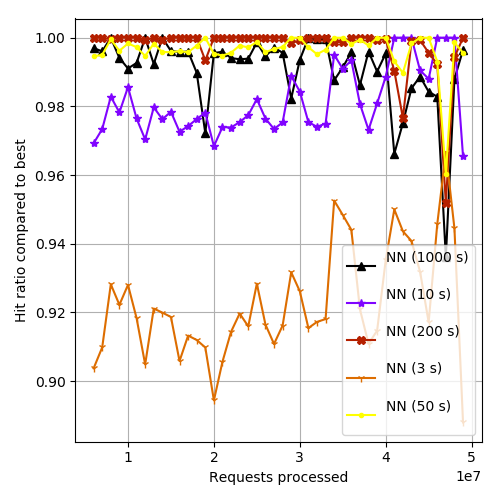
\includegraphics[width=\linewidth]{pics/cache7.png}
		\caption{5-day trace.}
	\end{subfigure}
	\begin{subfigure}[b]{0.49\linewidth}
		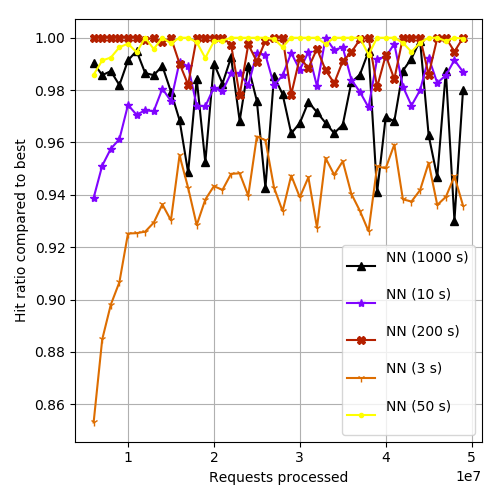
\includegraphics[width=\linewidth]{pics/cache7_2.png}
		\caption{30-day trace.}
	\end{subfigure}
	\caption{Comparison of immediate cache hit ratio for different time frame sizes.}
	\label{fig:cache7}
\end{figure}

Examining the cumulative hit rate revealed that the time frame size of 200 seconds performed the best. But studying closely the immediate hit rate, i. e. evaluating the hit rate after each million of requests rather than the total hit rate, revealed some interesting behavior. Figure \ref{fig:cache7} shows the ratio between the best-performing policy modification and other modifications evaluating immediate hit rate as described before for both of the real traces and cache size of 200. The figure reveals that the best-performing cumulatively time frame size does not perform the best at each point in time of the traces. At some segments of the traces, the 50 second size performs the best, what could be expected since this size was very close to the best-performing in all tests. More importantly, during some periods the size of 10 seconds performed the best. A close look at the segments of the traces on which the size of 10 seconds performed the best revealed that the rate of requests was very high. Correspondingly, a 10 second modification would estimate the popularity of the objects with high accuracy while being the fastest to adapt to the changes since it naturally follows from the smaller size of the time frame. Such behavior suggests that possibly it is better to reject the concept of time-based time frames and switch to request based frames, i. e. the frame will not span a fixed amount of time but a fixed number of requests. Such an approach should remove the dependence on the request rate of the request trace and could allow simplifying the parameter selection for the policy. We have not tested such a modification and we leave it for future research.

We also tried improving the quality of predictions made by the neural network by passing as input some metadata alongside with the popularity in previous time frames, in our case, they were the size of the object and the time of the day, but they did not improve the performance of the policy. However, the approach of adding metadata to the input of the neural network should not be discarded. It is possible that some other metadata could improve the quality of predictions and the performance of the caching policy as consequence. Investigation on which metadata may be useful is left for future research.

\subsection{Computational and memory cost} \label{comp_mem_cost}

Having figured out the optimal way for parameter selection, we can now evaluate the computational cost and memory footprint introduced by our solution. 

We will start with the analysis by the memory footprint. Our policy is relying on a neural network. The memory footprint of the neural network is the memory footprint of its weights. Denoting the number of neurons in the input layer as $a$, in hidden layers as $b$, in the output layer as $c$, and number of hidden layers as $n$, and assuming the connections are represented as double-precision floating point numbers, brings the total memory footprint of the neural network to be:
$$ (a * b + b^2 * (n - 1) + b * c) * 8 \text{ bytes } $$
In Section \ref{chosen_architecture} we have discussed the architecture of the neural network. We chose the architecture with 4 neurons in the input layer, this choice has been confirmed to be optimal in Section \ref{parameter_selection}, 2 hidden layers with 128 neurons in each and 1 neuron in the output layer. Adding to this an extra neuron to the input layer which takes the time fraction of the current time frame, discussed in Section \ref{nn_online}, and an extra bias neuron for each layer except the output brings the total memory footprint of our neural network architecture to be:
$$ (6 * 129 + 129^2 * (2 - 1) + 129 * 1) * 8 = 140352 \text{ bytes } \approx 140 \text{ kB } $$
The policy also requires to keep track of popularity, i.e. number of requests, for each object. Assuming the worst case scenario, each request in the time window is a unique object. Counter for each item is assumed to consume 12 bytes, 8 bytes ID and 4 bytes counter itself. Denoting the average number of requests per window as $x$ and the number of windows for prediction as $y$, gives the total memory footprint of:
$$ x * y * 12 \text{ bytes } $$
Using recommended parameters brings the total number of requests in a time frame to be around $ 180000 $. Accounting for 4 to be recommended number of  windows, brings the total memory footprint for keeping track for content popularity to be:
$$ 180000 * 4 * 12 = 8640000 \text{ bytes } = 8640 \text{ kB } $$
Finally, to train the neural network the policy requires to keep training datasets for $k$ previous time frames, as explained in section \ref{online_learning}. This number can be regulated using parameters $\alpha$ and forget threshold. Each row of the dataset has $x + 2$ floating point numbers, amounting to $(x + 2) * 8$ bytes per row. One request adds a row to the dataset, thus the memory footprint of keeping training datasets in memory:
$$ k * x * (x + 2) * 8 \text{ bytes } = 86400000 \text{ bytes } = 86400 \text{ kB }$$
Again, using the recommended parameters:
$$ 10 * 180000 * (4 + 2) * 8 = 86400000 \text{ bytes } = 86400 \text{ kB }$$
Adding to this the requirement to maintain a priority queue, which consumes $16 * C$ bytes, brings the total memory footprint to be:
$$ 140 \text{ kB } + 8640 \text{ kB } + 86400 \text{ kB } + 16 * C \text{ B } = 95180 \text{ kB } + 16 * C { B } $$
This number can be further decreased by switching to single-precision floating point numbers. In this way, the contribution of the highest contributing member to the total footprint would be halved.

Moving on with the calculation of the computational cost, the first contributing member is the maintenance of the priority queue with time complexity of $ O(\log\,C) $. The second contributing member is the complexity introduced by the neural network. Propagation of the input from one layer of the network to another has a complexity of $ O(m*l) $ where $m \text{ and } l$ are number of neurons in these layers. Using previously established notation, one full propagation through a neural network gives the complexity of $ O(a*b + (n-1)*b + b*c)$. In Section \ref{architecture} we discussed the requirement to update the popularity for a few objects at each cache hit, let's denote this number as $l$. Since each update requires the propagation through the neural network and accounting for previously discussed complexity of priority queue gives the total time complexity of our proposed approach to be: $$ O(l * (\log \, C + a*b + (n-1)*b + b*c)) $$

%Moving on with the calculation of the computational cost, we have proposed fixed values for each of the performance-influencing variables. Thus, only the size of the cache is the influencing factor to the time complexity. Cache size influences only the performance of the priority queue, thus, the time complexity is $ O(\log\,C) $, but with a much larger constant than in case of ARC or LRU. If we assume that the architecture of the neural network is also variable, we need to account for matrix multiplication involved in input propagation through the neural network. This adds roughly $ O(n^3) $ to the time complexity, where $n$ is the number of neurons in the largest layer of the network, bringing the total complexity to be $$  $$

\subsection{Comparison with other proposed solutions} \label{comparison}

\begin{figure}[b!]
	\centering
	\captionsetup{justification=centering}
	
	\begin{subfigure}[b]{0.49\linewidth}
		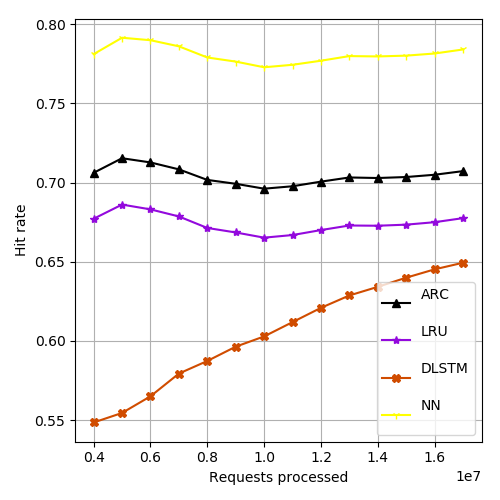
\includegraphics[width=\linewidth]{pics/dlstm_cum1.png}
		\caption{\% of cumulative hit rate.}
	\end{subfigure}
	\begin{subfigure}[b]{0.49\linewidth}
		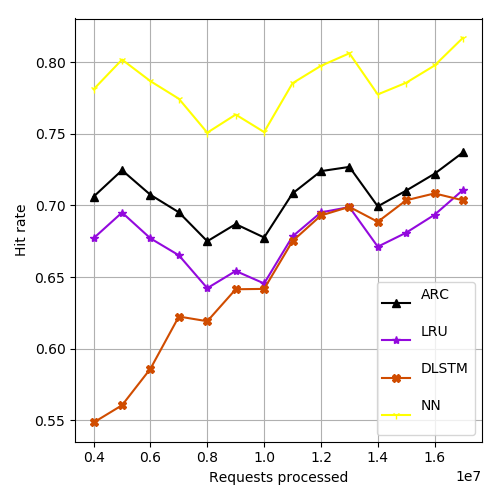
\includegraphics[width=\linewidth]{pics/dlstm_i1.png}
		\caption{\% of immediate hit rate.}
	\end{subfigure}
	
	\begin{subfigure}[b]{0.49\linewidth}
		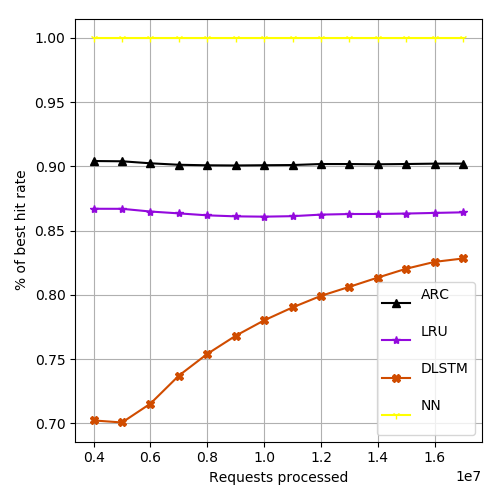
\includegraphics[width=\linewidth]{pics/dlstm_cum.png}
		\caption{\% of cumulative hit rate.}
	\end{subfigure}
	\begin{subfigure}[b]{0.49\linewidth}
		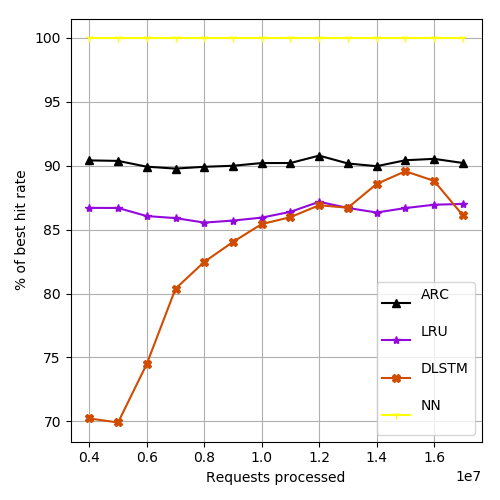
\includegraphics[width=\linewidth]{pics/dlstm_i.png}
		\caption{\% of immediate hit rate.}
	\end{subfigure}

	\caption{Comparison of performance of DLSTM policy with other policies on 5-day trace.}
	\label{fig:dlstm}
\end{figure}

We have shown before that our proposed caching policy overperform well established and frequently used policy LRU and industry leader policy ARC by close to 12\% and 3\% in absolute cache hit ratio and by 75-25\% and 11-5\% in relative cache hit ratio (depending on cache size) respectfully. But, as mentioned before, there are some proposed policies which also rely on machine learning algorithms for caching purposes. We have selected the approach proposed in \cite{23} to compare with the method proposed by us. As explained before, the policy proposed in \cite{23} applies deep long short-term memory network to determine the caching priority and decide which objects to store/remove in/from the cache. We have implemented the policy using the PyTorch library, which was also used to implement the neural network in our approach. DLSTM approach deals with a fixed number of items, so we filtered the 5-day trace to contain only $300 000$ most popular objects. After selecting the parameters of the policy as proposed by the author of \cite{23}, we evaluated the hit rate on our filtered trace. The produced hit rate values were less than 1\%. Probably, poor performance is caused by the inability of the neural network to tune all of its weights without a substantial number of iterations which is impossible to achieve while keeping performance suitable for the online task. And one-hot encoding utilized by DLSTM policy keeps the number of weights very high ($4.6 * 10^6$ weights between second hidden and output layers) increasing the impact of the problem. We reduced the number of unique items to 1000 and repeated the experiment, now with a better result shown in the Figure \ref{fig:dlstm}. The policy is showing some promise as can be seen by the upward trend in the cumulative cache hit ratio but the slow speed of adaptation at the first half of the trace caused a lower final cache hit ratio than achieved by ARC or our approach. Adding the disadvantage of a limited number of unique items to the slow adaptation speed of DLSTM policy we can claim that our approach is superior to the one proposed in \cite{23}.

